\chapter{Bitcoin Attacks}

Naive attempts to double spending are easily detected and rejected by the network.
By sending two transactions that spend the same coin, the network will accept only one of them, the first one that arrives. The second transaction will be rejected as it tries to spend a coin that has already been spent.
Or, still, adding the same coin two times in the same block will be rejected by the network, as the block is invalid.\\
However, there are more sophisticated attacks that can be performed on the Bitcoin network. In this chapter we will discuss some of them.

\section{51\% Attack}
\label{sec:51-attack}
\begin{paracol}{2}
   \colfill
   This attacks addresses the double spending problem by controlling the majority of the network's mining power.
   The attacker can then create a ``hidden'' fork of the blockchain, where the transaction that he wants to double spend is not included.
   He avoid broadcasting its fork until his chain is longer than the main chain, where he had spent its coins. At that point, he can broadcast his fork ---where he still owns its Bitcoins!--- and the network will accept it as the longest chain.
   \colfill
   \switchcolumn

   \begin{figure}[htbp]
      \centering
      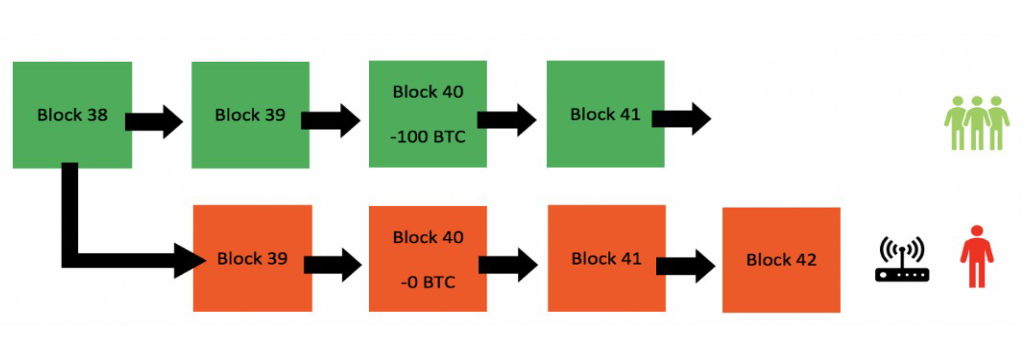
\includegraphics{images/bitcoin_atk511.png}\\
      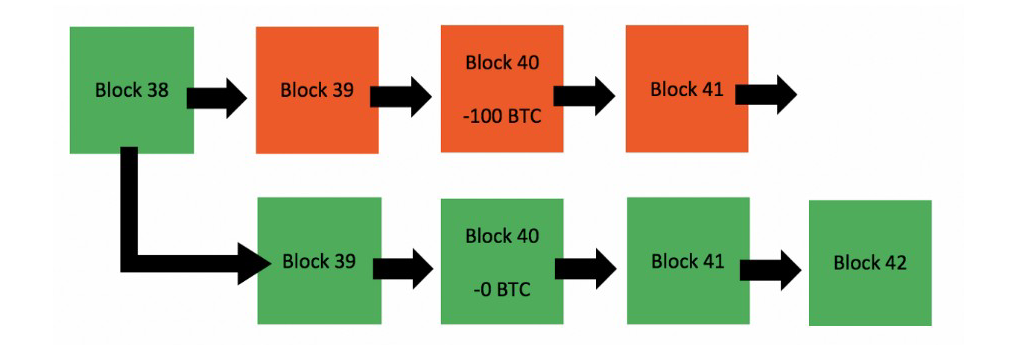
\includegraphics{images/bitcoin_atk512.png}
      \caption{Bitcoin 51\% Attack}
      \label{fig:bitcoin_atk51}
   \end{figure}
\end{paracol}

This attack requires for the attacker to control more than 50\% of the whole network's mining power, which is a \textit{very difficult} task. It is pretty unlikely that an attacker succeeds.

In 2014 GHash.io, a mining pool, reached 51\% of the network's mining power. The pool was asked to reduce its power, and it did.\\